% Rede neural em camadas (perceptron multicamadas)
% Feito para o ÉguaTeX (eguatex.com.br). Uso livre (CC0 1.0).
%
% Compile e pronto: sai só a figura, em PDF.
% Para pôr no seu trabalho, use o PDF com \includegraphics ou copie
% o bloco tikzpicture para dentro de uma figure.
\documentclass[tikz,border=4pt]{standalone}
\usepackage[T1]{fontenc}
\usepackage{lmodern}

\colorlet{corEntrada}{blue!20}
\colorlet{corOculta}{black!8}
\colorlet{corSaida}{red!20}

\begin{document}
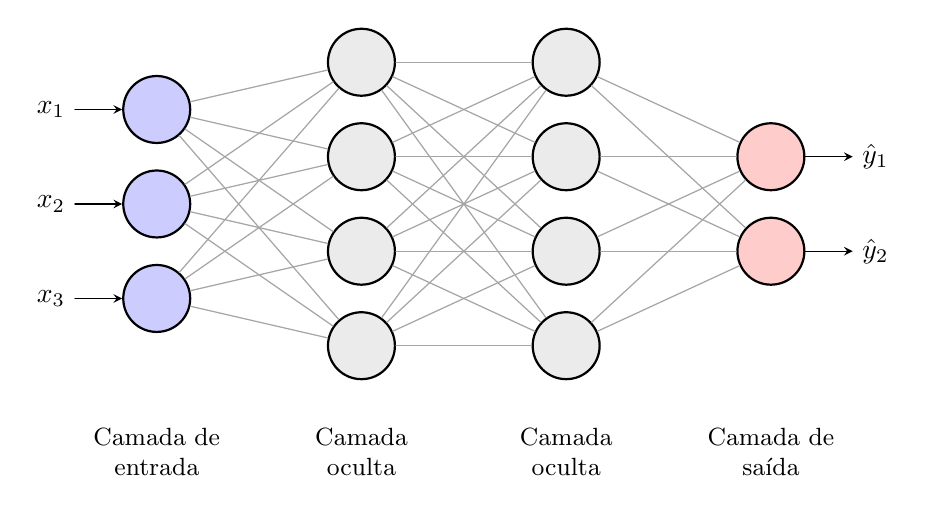
\begin{tikzpicture}[line cap=round,
  neuronio/.style={circle, draw, line width=0.8pt, minimum size=0.85cm, inner sep=0pt},
  ligacao/.style={black!35, line width=0.45pt}]

% Mude o número de neurônios de cada camada, da entrada para a saída.
\def\camadas{3,4,4,2}
\def\dx{2.6}  % distância entre camadas, em cm
\def\dy{1.2}  % distância entre neurônios, em cm

\def\maior{0}
\foreach \n [count=\c] in \camadas {\xdef\total{\c}\ifnum\n>\maior \xdef\maior{\n}\fi}

% neurônios
\foreach \n [count=\c] in \camadas {
  \foreach \i in {1,...,\n} {
    \ifnum\c=1 \def\cor{corEntrada}\else\ifnum\c=\total \def\cor{corSaida}\else \def\cor{corOculta}\fi\fi
    \node[neuronio, fill=\cor] (n-\c-\i) at ({(\c-1)*\dx},{(\n+1)/2*\dy-\i*\dy}) {};
  }
  \xdef\ultimo{\n}
}

% ligações entre camadas vizinhas
\foreach \n [count=\c, remember=\n as \m (initially 0)] in \camadas {
  \ifnum\c>1
    \pgfmathtruncatemacro{\ant}{\c-1}
    \foreach \i in {1,...,\m} \foreach \j in {1,...,\n}
      \draw[ligacao] (n-\ant-\i) -- (n-\c-\j);
  \fi
}

% rótulos de entrada, de saída e das camadas
\foreach \n [count=\c] in \camadas {
  \ifnum\c=1
    \foreach \i in {1,...,\n} \draw[<-, >=stealth] (n-1-\i.west) -- ++(-0.6,0) node[left] {$x_{\i}$};
    \node[font=\small, align=center] at ({(\c-1)*\dx},{-(\maior+1)/2*\dy-0.15}) {Camada de\\entrada};
  \else\ifnum\c=\total
    \foreach \i in {1,...,\n} \draw[->, >=stealth] (n-\c-\i.east) -- ++(0.6,0) node[right] {$\hat{y}_{\i}$};
    \node[font=\small, align=center] at ({(\c-1)*\dx},{-(\maior+1)/2*\dy-0.15}) {Camada de\\saída};
  \else
    \node[font=\small, align=center] at ({(\c-1)*\dx},{-(\maior+1)/2*\dy-0.15}) {Camada\\oculta};
  \fi\fi
}
\end{tikzpicture}
\end{document}
